\ylDisplay{Litter} % Ülesande nimi
{Tundmatu autor} % Autor
{lõppvoor} % Voor
{2012} % Aasta
{P 9} % Ülesande nr.
{3} % Raskustase
{
% Teema: Mehaanika

\ifStatement
Joonisel on kujutis, mille jättis pealtvaates pika säriajaga tehtud fotole lambike, mis oli kinnitatud jääl hõõrdevabalt libisevale ja pöörlevale kettakujulisele litrile. Lambi kinnituskoht asub $a = 4,5$ cm kaugusel litri püstteljest. Lamp põleb tuhmilt siniselt, kuid vilgatab  iga $t = 0,10$ s järel heledamalt punaselt. Fotole on lisatud tundmatu sammuvahega ruudustik. Leidke litri edasiliikumiskiirus.
\begin{center}
	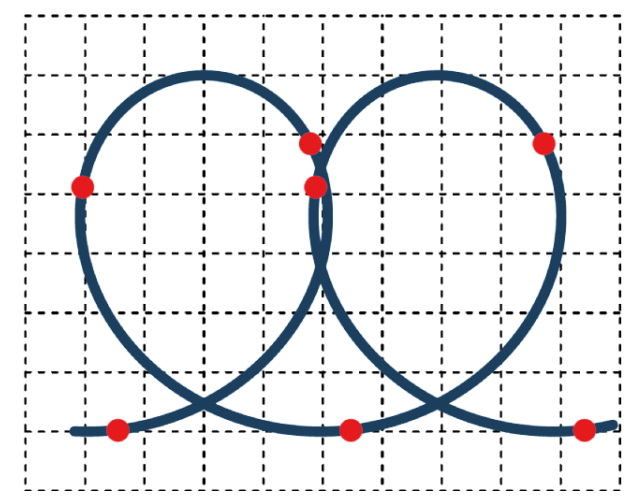
\includegraphics[width=0.5\linewidth]{2012-v3p-09-yl.PNG}
\end{center}
\fi

\ifHint
Sellest, et trajektoori madalaima ja kõrgeima punkti vahe vertikaalsuunas peab olema $2a$, saame leida ruudustiku sammuvahe.
\fi

\ifSolution
Esmalt paneme tähele, et trajektoori madalaima ja kõrgeima punkti vahe vertikaalsuunas peab olema $2a$, joonisel loeme selleks kuus ruutu, seega on ruudustiku sammuvahe $triangle = 2a/6 = 1,5$ cm. Teiseks paneme tähele, et iga pöörlemisperioodi järel kordub küll trajektoori kuju, kuid see nihkub horisontaalsuunas nelja ruudu võrra. Seega läbib litter pöörlemisperioodi jooksul vahemaa $s = 4\triangle = 6,0$ cm. Kolmandaks märkame, et pöörlemisperioodi sisse mahub täpselt kolm punaste vilgatuste vahelist intervalli, seega on pöörlemisperioodi kestus $T = 3t = 0,30$ s. Neist andmeist saame litri edasiliikumiskiiruseks $v = \frac{s}{T} = 20$ cm/s.
\fi
}
